%%%%%%%%%%%%%%%%%%%%%%%%%%%%%%%%%%%%%%%%%%%%%%%%%%%%%%%%%%%% 
% Name: XeTeX+xeCJK日常使用模板
% Author: Lox Freeman
% Email: xiaohanyu1988@gmail.com
% 、
% 本文档可以自由转载、修改,希望能给广大TeXer的中文之路提供一些方便。
%%%%%%%%%%%%%%%%%%%%%%%%%%%%%%%%%%%%%%%%%%%%%%%%%%%%%%%%%%%% 

\documentclass[a4paper, 12pt, titlepage]{article}

%%%%%%%%%%%%%%%%%%%%%%%%% xeCJK相关宏包%%%%%%%%%%%%%%%%%%%%%%%%%
\usepackage{xltxtra,fontspec,xunicode}
\usepackage[slantfont, boldfont, CJKchecksingle]{xeCJK}

\CJKsetecglue{\hskip 0.15em plus 0.05em minus 0.05em}
% slanfont: 允许斜体
% boldfont: 允许粗体
% CJKnormalspaces: 仅忽略汉字之间的空白,但保留中英文之间的空白。
% CJKchecksingle: 避免单个汉字单独占一行。
% CJKaddspaces: [备选]忽略汉字之间的空白,并且自动在中英文转换时插入空白。

% \CJKlanguage{zh-cn}                 % 中文标点特殊处理
\XeTeXlinebreaklocale "zh"           % 针对中文进行断行
\XeTeXlinebreakskip = 0pt plus 1pt minus 0.1pt
% 给予TeX断行一定自由度
%%%%%%%%%%%%%%%%%%%%%%%%% xeCJK%%%%%%%%%%%%%%%%%%%%%%%%%%%%%%%%

%%%%%%%%%%%%% 日常所用宏包、通通放在一起%%%%%%%%%%%%%%%%%%%%%%%%%%%%
% 什么常用的宏包都可以放这里。下面是我常用的宏包,每个都给出了简要注释
\usepackage[top=2.5cm, bottom=3cm, left=2.5cm, right=2.5cm]{geometry} % 控制页边距
\usepackage{enumerate}               % 控制项目列表
\usepackage{multicol}                % 多栏显示

\usepackage[%
pdfstartview=FitH,%
CJKbookmarks=true,%
bookmarks=true,%
bookmarksnumbered=true,%
bookmarksopen=true,%
colorlinks=true,%
citecolor=seco,%
linkcolor=seco,%
anchorcolor=seco,%
urlcolor=seco%
]{hyperref}                          % 超链接相关设置

\usepackage{titlesec}                % 控制标题
\usepackage{titletoc}                % 控制目录
\usepackage{type1cm}                 % 控制字体大小
\usepackage{indentfirst}             % 首行缩进,用\noindent取消某段缩进
\usepackage{bbding}                  % 一些特殊符号
\usepackage{cite}                    % 支持引用
\usepackage{framed,color,xcolor}     % 支持彩色文本、底色、文本框等
\usepackage{latexsym}                % LaTeX一些特殊符号宏包
\usepackage{amsmath}                 % AMS LaTeX宏包
\usepackage{bm}                      % 数学公式中的黑斜体
\usepackage{relsize}                 % 调整公式字体大小:\mathsmaller, \mathlarger
\usepackage{soul}                    % 下划线自动回车换行
\usepackage{attachfile}              % 添加附见使用的宏包
\usepackage{parcolumns}              % 列排版
\usepackage{framed}
\usepackage{tcolorbox}
\usepackage{pdfpages}                % 直接引用已有的PDF文件
\usepackage{soul}                    % 自动换行的下划线
\makeindex                           % 生成索引

\makeatletter
\let\std@footnotetext\@footnotetext
\usepackage{setspace}
\let\@footnotetext\std@footnotetext
\makeatother

%%%%%%%%%%%%%%%%%%%%%%%%% 绘图方法%%%%%%%%%%%%%%%%%%%%%%%%%%%
\usepackage{graphicx}                % 图形宏包
\graphicspath{{./figure/}{./figures/}{./image/}{./graphics/}{./graphic/}{./pictures/}{./picture/}}

\usepackage{tikz}
\usepackage{amsmath,bm,times}
\usepackage{verbatim}

\usepackage{tabularx}

\usetikzlibrary{shapes,arrows,shadows,fit,snakes,positioning,decorations}
\usetikzlibrary{decorations.shapes}
\usetikzlibrary{calc}           %coordinate

\usepackage{caption}
\usepackage{float}

\ifx\du\undefined
\newlength{\du}
\fi
\setlength{\du}{15\unitlength}

\newlength\Textwd
\setlength\Textwd{3cm}
\newcommand\Textbox[2]{%
  \parbox[c][#1][c]{\Textwd}{\linespread{0.5}\centering#2}}

\makeatletter
\DeclareRobustCommand{\rvdots}{%
  \vbox{
    \baselineskip6\p@\lineskiplimit\z@
    \kern-\p@
    \hbox{.}\hbox{.}\hbox{.}
  }}
\makeatother


\makeatletter
\DeclareRobustCommand{\rvdots}{%
  \vbox{
    \baselineskip4\p@\lineskiplimit\z@
    \kern-\p@
    \hbox{.}\hbox{.}\hbox{.}}}
\tikzset{
  heights/.code={
    \def\pgf@tempb{}%
    \foreach \qrr@tikz@rs@height[count=\qrr@tikz@count from 1] in {#1}{
      \edef\pgf@tempa{\noexpand\pgfkeysalso{/tikz/every \pgf@lib@sh@toalpha\qrr@tikz@count\space node part/.append style={height={\qrr@tikz@rs@height}}}}%
      \ifnum\qrr@tikz@count=1\relax % allows to use \nodepart{text} (or not at all for the first part)
      \edef\pgf@tempa{\unexpanded\expandafter{\pgf@tempa}\noexpand\pgfkeysalso{/tikz/every text node part/.append style={height={\qrr@tikz@rs@height}}}}%
      \fi
      \expandafter\pgfutil@g@addto@macro\expandafter\pgf@tempb\expandafter{\pgf@tempa}
    }
    \pgf@tempb
  },
  height/.code={%
    \expandafter\def\expandafter\pgfutil@minipage\expandafter[\expandafter##\expandafter 1\expandafter]\expandafter{\pgfutil@minipage[][#1][c]}% LaTeX only!
  }
}

\makeatother
\tikzset{rect/.style={
    draw,
    rectangle split,
    rectangle split parts=1,
    rectangle split part align=center,
    draw,
    % font=\ttfamily, % still works
    thick,
    text width=2.5cm,
    align=center,
    rectangle split part align={center,left,right},
    % rectangle split part fill={PaleTurquoise1},
  }}

\makeatletter
\newcommand{\gettikzxy}[3]{%
  \tikz@scan@one@point\pgfutil@firstofone#1\relax
  \edef#2{\the\pgf@x}%
  \edef#3{\the\pgf@y}%
}
\makeatother
%%%%%%%%%%%%%%%%%%%%%%%%% 绘图方法结束%%%%%%%%%%%%%%%%%%%%%%%%%%%

%%%%%%%%%%%%%%%%%%%%%%%%% fancyhdr设置页眉页脚%%%%%%%%%%%%%%%%%%%%
\usepackage{etoolbox}
\usepackage{fancyhdr}                % 页眉页脚
\pagestyle{fancy}                    % 页眉页脚风格
\setlength{\headheight}{15pt}        % 有时会出现\headheight too small的warning

\makeatletter
\patchcmd{\@fancyhead}{\rlap}{\color{seco}\rlap}{}{}
\patchcmd{\headrule}{\hrule}{\color{seco}\hrule}{}{}
\patchcmd{\@fancyfoot}{\rlap}{\color{seco}\rlap}{}{}
\patchcmd{\footrule}{\hrule}{\color{seco}\hrule}{}{}
\makeatother
%%%%%%%%%%%%%%%%%%%%%%%%% fancyhdr设置结束%%%%%%%%%%%%%%%%%%%%%%%

%%%%%%%%%%%%%%%%%%%%%%%%% xeCJK字体设置%%%%%%%%%%%%%%%%%%%%%%%%%
% \setmainfont[Ligatures=TeX]{Minion Pro} % (\textrm)
\setmainfont[Ligatures=TeX]{Calibri} % (\textrm)
% \setsansfont{Myriad Pro}                % (\textsf)
\setsansfont{Calibri}                % (\textsf)
% \setmonofont{Adobe Garamond Pro}        % Palatino Linotype
\setmonofont{Ubuntu Mono}        % Palatino Linotype

\setCJKmainfont[BoldFont={方正兰亭纤黑_GBK},ItalicFont={Adobe Kaiti Std}]{Adobe Kaiti Std}
\setCJKsansfont[BoldFont={方正兰亭纤黑_GBK}]{方正兰亭纤黑_GBK}
\setCJKmonofont{方正兰亭纤黑_GBK}
%%%%%%%%%%%%%%%%%%%%%%%%% xeCJK字体设置结束%%%%%%%%%%%%%%%%%%%%%%

%%%%%%%%%%%%%%%%%%%%%%%%% listings宏包粘贴源码%%%%%%%%%%%%%%%%%%%%
\usepackage{listings}                % 方便粘贴源代码,部分代码高亮功能
\lstloadlanguages{}                  % 所要粘贴代码的编程语言

\newfontfamily\listingsfont{Ubuntu Mono}
\newfontfamily\listingsfontinline{Calibri}

\definecolor{sh_keyword}{rgb}{0.06, 0.10, 0.98}   % #101AF9
\definecolor{shadecolor}{rgb}{0.83, 0.83, 0.83}
\definecolor{monokai-grey-dark}{RGB}{39, 40, 34}   % #272822
\definecolor{monokai-yellow-light}{RGB}{248, 248, 246}   % #F8F8F2
\definecolor{monokai-green}{RGB}{166, 226, 42}
\definecolor{dark green}{rgb}{0.000000,0.392157,0.000000}
\definecolor{forest green}{rgb}{0.133333,0.545098,0.133333}
\def\lstsmallmath{\leavevmode\ifmmode \scriptstyle \else  \fi}
\def\lstsmallmathend{\leavevmode\ifmmode  \else  \fi}

% \definecolor{seco}{RGB}{9,80,3}
% \definecolor{seco}{RGB}{0,145,215}
\definecolor{seco}{RGB}{0,175,152}
\definecolor{main}{RGB}{127,191,51}

% \makeatletter
%   \newcommand\listingfont{\@setfontsize\listingfont{11pt}{13.2pt}}
% \makeatother

\renewcommand{\lstlistingname}{代码}

\lstset {
  language=c++,
  backgroundcolor=\color{monokai-grey-dark},
  % frame=shadowbox,
  % breaklines,
  % rulesepcolor=\color{red!20!green!20!blue!20},
  showspaces=false,showtabs=false,tabsize=4,
  numberstyle=\tiny\color{black},numbers=left,
  % basicstyle= \listingfont\listingsfont\color{monokai-yellow-light},
  basicstyle= \small\listingsfont\color{monokai-yellow-light},
  stringstyle=\color{dark green},
  % keywordstyle = \color{monokai-green}\bfseries,
  keywordstyle = \color{monokai-green},
  commentstyle=\footnotesize\color{forest green}\itshape,
  captionpos=b,
  showspaces=false,showtabs=false, showstringspaces=false,
  xleftmargin=0.7cm, xrightmargin=0.5cm,
  % lineskip=-0.3em,
  breaklines=tr,
  escapebegin={\lstsmallmath}, escapeend={\lstsmallmathend},
  extendedchars=false
}

\lstnewenvironment{acol}[1][]{\lstset{language={[x86masm]Assembler},#1}}{}
\newenvironment{parcolumenv}[1] {\begin{spacing}{#1}}{\end{spacing}}
%%%%%%%%%%%%%%%%%%%%%%%%% listings宏包设置结束%%%%%%%%%%%%%%%%%%%%


%%%%%%%%%%%%%%%%%%%%%%%%% 一些关于中文文档的重定义%%%%%%%%%%%%%%%%%

%%%% 数学公式定理的重定义%%%%
\newtheorem{example}{例}                                   % 整体编号
\newtheorem{algorithm}{算法}
\newtheorem{theorem}{定理}[section]                        % 按 section 编号
\newtheorem{definition}{定义}
\newtheorem{axiom}{公理}
\newtheorem{property}{性质}
\newtheorem{proposition}{命题}
\newtheorem{lemma}{引理}
\newtheorem{corollary}{推论}
\newtheorem{remark}{注解}
\newtheorem{condition}{条件}
\newtheorem{conclusion}{结论}
\newtheorem{assumption}{假设}

%%%% 章节等名称重定义%%%%
\renewcommand{\contentsname}{目\hspace{2em}录}
\renewcommand{\indexname}{索引}
\renewcommand{\listfigurename}{插图目录}
\renewcommand{\listtablename}{表格目录}
\renewcommand{\figurename}{图}
\renewcommand{\tablename}{表}
\renewcommand{\appendixname}{附\hspace{2em}录}

%%%% 设置chapter、section与subsection的格式%%%%
\titleformat{\chapter}{\centering\huge}{\color{seco}第\thechapter{}章}{1em}{\color{seco}\textbf}
\titleformat{\section}{\centering\LARGE}{\color{seco}\thesection}{1em}{\color{seco}\textbf}
\titleformat{\subsection}{\Large}{\color{seco}\thesubsection}{1em}{\color{seco}\textbf}
%%%%%%%%%%%%%%%%%%%%%%%%% 中文重定义结束%%%%%%%%%%%%%%%%%%%%


%%%%%%%%%%%%%%%%%%%%%%%%% 一些个性设置%%%%%%%%%%%%%%%%%%%%%%
\setlength{\parskip}{0.5\baselineskip}     % 设定段间距
\linespread{1.6}                           % 设定行距
\newcommand{\pozhehao}{\kern0.3ex\rule[0.8ex]{2em}{0.1ex}\kern0.3ex}% 中文破折号,据说来自清华模板

\setCJKfamilyfont{title}{方正正中黑简体}

\newcommand*{\TitleFont}{\usefont{\encodingdefault}{\rmdefault}{b}{n}\fontsize{32}{40}\selectfont\CJKfamily{title}\color{seco}}% 标题字体设置

\renewcommand{\today}{\color{seco}\number\year 年 \number\month 月 \number\day 日}
%%%%%%%%%%%%%%%%%%%%%%%%% 个性设置结束%%%%%%%%%%%%%%%%%%%%%%


%%%%%%%%%%%%%%%%%%%%%%%%% 正文部分%%%%%%%%%%%%%%%%%%%%%%%%%
\begin{document}
\setlength{\parindent}{2em}

\title{\TitleFont 也谈C++的虚函数表\vspace{8cm}}
\author{\href{mailto:q00148943@gmail.com}{\LARGE{秦新良}}}
\date{\vspace{0.5cm}\today}

\maketitle

\tableofcontents
\newpage

\section{缘起}
从\href{http://blog.csdn.net/haoel/article/details/1948051}{C++虚函数表解析}这篇文章中我们可以了解到,C++中的虚函数是通过一张虚函数表来实现的。如图\ref{fig1}所示,基类\emph{Base}实例化后,其隐含的指针\emph{*\_\_vptr}指向了\emph{Base}的虚函数表。

\begin{figure}[!htb]
  \setlength{\abovecaptionskip}{0pt}
  \begin{center}
    \begin{singlespace}
      \begin{tikzpicture}[auto,
        rect/.style={
          rectangle split, rectangle split parts=3,
          draw,rectangle split part align=center,draw, thick,
          text width=3cm,
          text centered, %minimum height=26em,
          align=center, rectangle split part align={center,left},
          rectangle split part align=midway,
          rectangle split part fill={green!30, blue!20, gray!30, blue!15, blue!20,blue!15,blue!15,green!15,green!20}
        }]

        % Split Rectangle
        \node (instance) [rect] {
          \nodepart {one} \Textbox{}{\footnotesize *\_\_vptr}
          \nodepart {two} \Textbox{}{\footnotesize data\ member}
          \nodepart{three} \Textbox{}{\scriptsize \rvdots}
        };

        \tikzset{horizon_rect/.style={
            draw,
            rectangle split,
            rectangle split horizontal,
            rectangle split empty part height=2cm,
            rectangle split parts=9,
            draw,
            thick,
            text width=2.5cm,
            % text height=1cm,
            align=center,
            rectangle split part align={center,left,right},
            rectangle split part fill={green!30},
          }}

        \node (vtable) [horizon_rect, right of=instance, rectangle split parts=4, xshift=6cm] {
          \nodepart[]{text} {\footnotesize{Base::$\sim$Base()}}
          \nodepart[]{two} {\footnotesize{Base::fun1()}}
          \nodepart[]{three} {\footnotesize{Base::fun2()}}
          \nodepart[text width=0.5cm]{four} {\footnotesize{.}}
        };

        \draw [-latex,thick] ($(instance.text east) + (0,0)$) -- ($(vtable.west) + (0,0)$);
        % node [draw=none,midway,below=0.3cm] {\footnotesize $iter$};

        \node[yshift=1pt,anchor=south] at (instance.north) {\scriptsize $A\ instance\ of\ Base$};
        \node[yshift=1pt,anchor=south] at (vtable.north) {\scriptsize $virtual\ table\ for\ class\ Base$};

      \end{tikzpicture}
    \end{singlespace}
  \end{center}
  \caption{Base的虚函数表}
  \label{fig1}
\end{figure}

\noindent 当基类\emph{Base}被派生类\emph{D1}继承并覆盖其虚函数\emph{fun1}后,\emph{D1}实例化后的隐含指针\emph{*\_\_vptr}与其虚函数表的关系如图\ref{fig2}所示。

\begin{figure}[!htb]
  \setlength{\abovecaptionskip}{0pt}
  \begin{center}
    \begin{singlespace}
      \begin{tikzpicture}[auto,
        rect/.style={
          rectangle split, rectangle split parts=3,
          draw,rectangle split part align=center,draw, thick,
          text width=3cm,
          text centered, %minimum height=26em,
          align=center, rectangle split part align={center,left},
          rectangle split part align=midway,
          rectangle split part fill={green!30, blue!20, gray!30, blue!15, blue!20,blue!15,blue!15,green!15,green!20}
        }]

        % Split Rectangle
        \node (instance) [rect] {
          \nodepart {one} \Textbox{}{\footnotesize *\_\_vptr}
          \nodepart {two} \Textbox{}{\footnotesize data\ member}
          \nodepart{three} \Textbox{}{\scriptsize \rvdots}
        };

        \tikzset{horizon_rect/.style={
            draw,
            rectangle split,
            rectangle split horizontal,
            rectangle split empty part height=2cm,
            rectangle split parts=9,
            draw,
            thick,
            text width=2.5cm,
            % text height=1cm,
            align=center,
            rectangle split part align={center,left,right},
            rectangle split part fill={green!30},
          }}

        \node (vtable) [horizon_rect, right of=instance, rectangle split parts=4, xshift=6cm] {
          \nodepart[]{text} {\footnotesize{D1::$\sim$D1()}}
          \nodepart[]{two} {\footnotesize{D1::fun1()}}
          \nodepart[]{three} {\footnotesize{Base::fun2()}}
          \nodepart[text width=0.5cm]{four} {\footnotesize{.}}
        };

        \draw [-latex,thick] ($(instance.text east) + (0,0)$) -- ($(vtable.west) + (0,0)$);
        % node [draw=none,midway,below=0.3cm] {\footnotesize $iter$};

        \node[yshift=1pt,anchor=south] at (instance.north) {\scriptsize $A\ instance\ of\ D1$};
        \node[yshift=1pt,anchor=south] at (vtable.north) {\scriptsize $virtual\ table\ for\ class\ D1$};
        
      \end{tikzpicture}
    \end{singlespace}
  \end{center}
  \caption{D1的虚函数表}
  \label{fig2}
\end{figure}
\noindent 类实例化后,其隐含的指针\emph{*\_\_vptr}是何时指向了类的虚函数表,类的虚函数表又是在什么时候初如化的?本文着重阐述这两个问题。
\section{虚函数表的初始化}
类实例化后,其隐含的指针\emph{*\_\_vptr}是何时指向了类的虚函数表?答案是编译器\footnote{本文验证使用的GCC版本为:gcc version 4.7.3 (Ubuntu/Linaro 4.7.3-1ubuntu1)}编译时在类的构造函数中自动插入了代码来做这个初始化的工作,这一点可以从\emph{Base}汇编后的构造函数中清楚的看到。\emph{Base}的定义如代码\ref{lst1}所示。代码\ref{lst2}为其编译后的汇编代码。\newline
\begin{spacing}{1.0}
  \lstinputlisting[label=lst1,caption=类的定义]{list/C1.cpp}
\end{spacing}

\begin{spacing}{1.0}
  \lstinputlisting[label=lst2,caption=Base的汇编代码,language={[x86masm]Assembler}]{list/base.s}
\end{spacing}

汇编代码中的\emph{\_ZN4BaseC1Ev}({\color{blue}4--9行})即为\emph{Base}的构造函数。第4和5行是每个函数开始执行的例行公事:保存上一个函数\footnote{调用该函数的函数,即调用者(caller)。}调用栈的栈基址,然后将本函数的栈基址保存到\emph{\%ebp}寄存器。第6行将构造函数的第一个入参\footnote{类的成员函数的第一个入参为{\color{blue}this}指针。}(即\emph{*\_\_vptr})存入寄存器\emph{\%eax},紧接着把地址{\color{red}0x80487d8}(基类\emph{Base}虚函数表的首地址)赋给\emph{\%eax}所指的内存,从而将\emph{*\_\_vptr}指向了类的虚函数表。同理可知,派生类\emph{D1}的虚函数表的首地址为{\color{red}0x80487c0}。

到这里我们清楚了类实例化后,\emph{*\_\_vptr}是如何初始化为虚函数表的首地址的。但这样还不足以说明\emph{*\_\_vptr}确实是指向了类的虚函数表,因为从上面的代码中根本看不出地址{\color{red}0x80487d8}和{\color{red}0x80487c0}就是虚函数表的地址。下面我们接着做进一步的验证。

通过\emph{objdump}解析二进制文件中的只读数据段的内容如图\ref{fig3}中的上半部分所示。解析后的只读数据段的首列是程序加载后的内存地址\footnote{程序运行过程中的逻辑地址。},紧接着后面4列是内存地址对应的值,每行16个字节。从图中可以看出,地址\emph{0x80487d8}的值为\emph{{\color{blue}d0850408}},因为笔者的系统是小端字节序的,转换过来就是\emph{{\color{blue}080485d0}}。从代码\ref{lst2}中可以找出\emph{{\color{blue}080485d0}}即为函数Base::$\sim$Base()的地址,即图\ref{fig3}中以红色椭圆标识部分。依次类推 ,地址\emph{0x80487dc}的值为\emph{{\color{blue}f8850408}},对应函数Base::$\sim$Base()\footnote{汇编代码中有两个析构函数。};地址\emph{0x80487e0}的值为\emph{{\color{blue}16860408}},对应函数Base::fun1();地址\emph{0x80487e4}的值为\emph{{\color{blue}1c860408}},对应函数Base::fun2();这样就构成了类Base的整张虚函数表。相信你也可以用样的方法推出类D1的虚函数表。
\begin{figure}[H]
  \setlength{\abovecaptionskip}{0pt}
  % \setlength{\belowcaptionskip}{10pt}
  \centering
  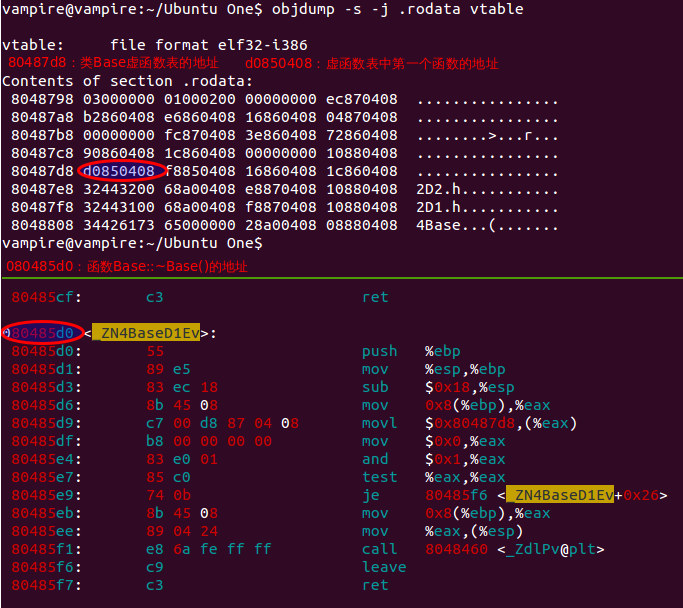
\includegraphics[width=0.99\textwidth]{vptr.png}
  \caption{虚函数表及虚函数}
  \label{fig3}
\end{figure}

\section{结论}
类的虚函数表在代码编译链接后即已确定,位于编译后二进制文件中的只读数据段;并且编译器会自动在类的构造函数中插入将\emph{*\_\_vptr}指向虚函数表的代码,从而实现类在实例化时自动将\emph{*\_\_vptr}赋值为类的虚函数表的首地址。

\end{document}
%%%%%%%%%%%%%%%%%%%%%%%%% 正文部分结束%%%%%%%%%%%%%%%%%%%%%%

